\documentclass[main.tex]{subfiles}
\begin{document}

\marginpar{Wednesday\\ 2020-12-9, \\ compiled \\ \today}

% We were discussing how the envelope of the neutron star can be treated in the plane-parallel approximation. 

% The conductivity tensor is 
% %
% \begin{align}
% k'_{ij} = \left[\begin{array}{cc}
% k_\parallel & 0 \\ 
% 0 & k_\perp
% \end{array}\right]
% \,,
% \end{align}
% %
% and so 
Therefore, the components of the tensor in the unprimed frame are 
%
\begin{align}
k_{ij} = \left[\begin{array}{cc}
k_\parallel \cos^2 \phi + k_\perp \sin^2\phi  & (k_\parallel - k_\perp) \sin \phi \cos \phi  \\ 
(k_\parallel - k_\perp) \sin \phi \cos \phi  & 
k_\parallel \sin^2 \phi + k_\perp \cos^2\phi
\end{array}\right]
\,,
\end{align}
%
which will be used in the law 
%
\begin{align}
q_i = - \sum _{j} k_{ij } \pdv{T}{x _j}
\,.
\end{align}

Since we are interested in the observable emission, 
let us consider \(q_z = q_2\), which will be given by 
%
\begin{align}
q_z = - k_{21} \pdv{T}{x} - k_{22} \pdv{T}{z}
\,,
\end{align}
%
and we know that this will correspond to blackbody emission: \(q_z = \sigma T^{4}\).

Now, as rough estimates, if \(L\) is the depth of the crust and \(R\) is the radius of the NS, we can take \(\pdv*{T}{z} \approx (T_s - T_c ) / L\), while \(\pdv*{T}{x} \approx - T_s/R\).

We know that \(T_s \ll T_c \), and \(L \ll R\): then, 
%
\begin{align}
\abs{ \pdv{T}{z}} \approx \abs{- \frac{T_0}{L} } \gg \pdv{T}{x}
\,.
\end{align}

So, taking only the most significant term we get 
%
\begin{align}
\sigma T^{4} &= - k_{22} \pdv{T}{z} = - \qty(
k_\parallel \sin^2 \phi + k_\perp \cos^2\phi) \pdv{T}{z}   \\
&= \underbrace{- k_\parallel \pdv{T}{z}}_{\sigma T_P^{4}} \qty( \sin^2 \phi + \frac{k_\perp}{k_\parallel} \cos^2 \phi )
\,,
\end{align}
%
where we defined the new temperature \(T_P\), since on dimensional grounds that term was a thermal emissivity. If we take \(\phi = \pi /2\) we get the temperature at the pole: therefore, \(T_P\) is the polar temperature.

As long as \(k_\perp \ll k_\parallel\), we get \(\sigma T^{4} \approx \sigma T_P^{4} \sin^2 \phi \).
We can also define the angle \(\Theta \), between \(\vec{B}\) and the radial direction, through \(\phi = \pi /2 - \Theta \).
% \footnote{This is not a bad approximation --- the correct geometrical considerations yield \(\phi = \arctan(2 / \tan \theta )\), which is only slightly different from \(\phi = \pi / 2 - \Theta \).}
% \todo[inline]{Is this true?}

This then tells us that \(T = T_P \sqrt{\abs{\cos \Theta }}\).
The dipolar magnetic field is given by 
%
\begin{align}
\vec{B} = \frac{B_p}{2} \qty(\frac{R}{r})^3 \qty(2 \cos \theta \hat{e}_r + \sin \theta \hat{e}_\theta )
\,,
\end{align}
%
so on the surface it will read
%
\begin{align}
\vec{B}(r = R) = \frac{B_p}{2} \qty(2 \cos \theta \hat{e}_r + \sin \theta \hat{e}_\theta )
\,.
\end{align}

The cosine of \(\Theta \), the angle between the \(\vec{B}\) field and the radial direction, is 
%
\begin{align}
\cos \Theta = \frac{\vec{B} \cdot \hat{e}_r}{\abs{\vec{B}}} = \frac{B_r}{B} = \frac{B_p}{2} \frac{2 \cos \theta }{B} 
\,,
\end{align}
%
so, taking geometric considerations into account, we get 
%
\begin{align}
\cos \Theta = \frac{2 \cos \theta }{\sqrt{1 + 3 \cos^2 \theta }}
\,.
\end{align}

Therefore, the temperature monotonically decreases going from the pole to the equator. 
At the equator it is not really zero, but it is an order of magnitude lower than the polar temperature. A plot of the approximated formula \(T/ T_P \sim \sqrt{\abs{\cos \Theta }}\) is shown in figure \ref{NS-temperature}.

\begin{figure}[H]
\centering
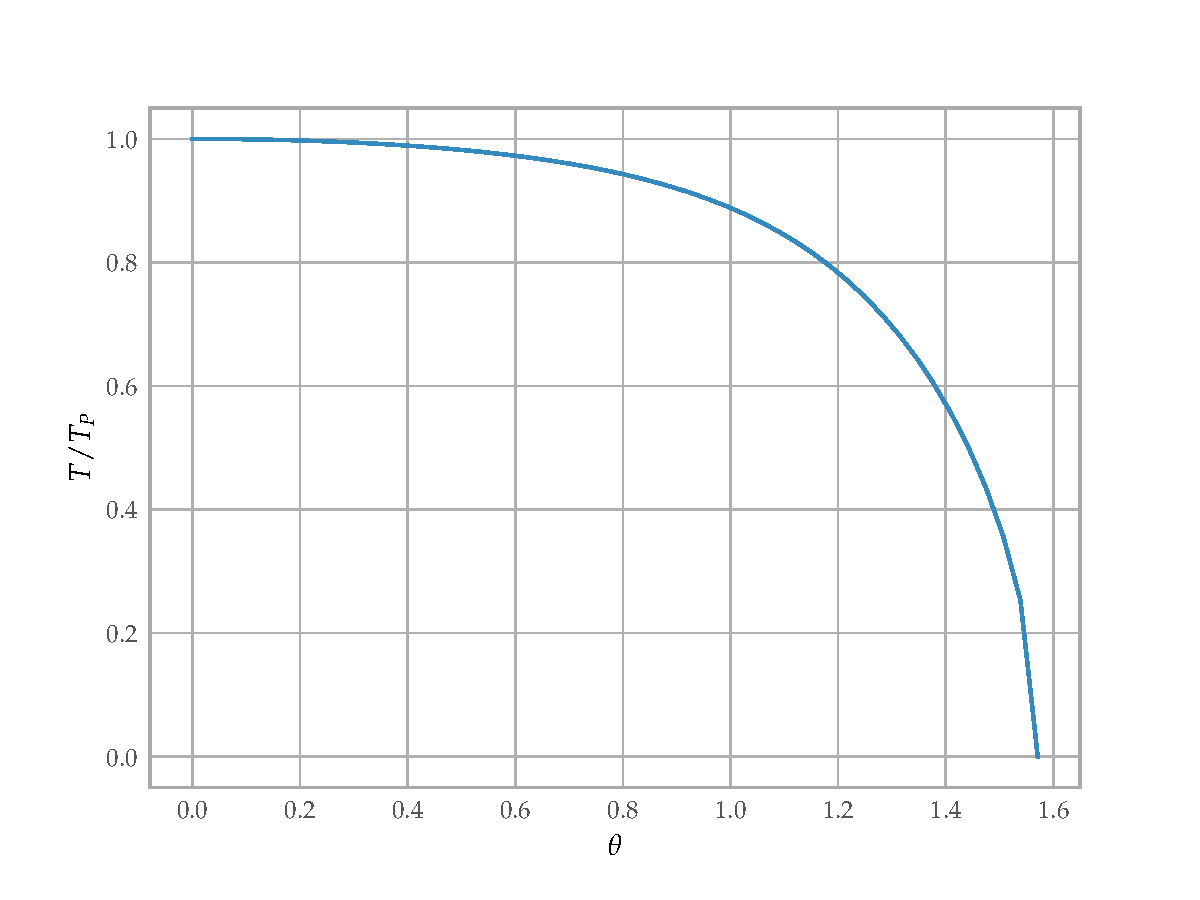
\includegraphics[width=.7\textwidth]{figures/NS-temperature}
\caption{Temperature as a function of \(\theta \). On the left we have the pole, on the right the equator; in reality the temperature will not drop to zero at \(\theta = \pi /2\), instead the conduction along \(x\) will become relevant.}
\label{fig:NS-temperature}
\end{figure}

This has an important observational implication: the emission from the NS is not a single blackbody, but instead a superposition of a blackbody for each latitude.

What we have done so far applies to the dipolar approximation, but nothing prevents higher order moments from being relevant. 

We also need to account for relativistic effects: 
\begin{enumerate}
    \item the emitted radiation is redshifted by a factor 
    %
    \begin{align}
    \frac{\nu _\infty}{\nu } = \sqrt{1 - \frac{2GM}{c^2R}} 
    \,,
    \end{align}
    %
    which typically comes out to \(\Delta \nu / \nu \sim \num{.2}\). This is reflected in a lower effective blackbody temperature.
    \item The luminosity at infinity is multiplied by a factor \((1 - 2GM/c^2R)\) compared to the one at the surface, because of the relativistic correction to the radius (\(R = R_\infty \sqrt{1 - 2GM/c^2R}\)), which factors into the surface area. 
    \item The light rays' paths will be curved by the gravitational effect of the NS. Consider the point of emission of a photon on the surface, and denote as \(\alpha \) the angle between the radial direction at that point and the direction of emission; further, denote as \(\theta \) the angle between the radial direction and our line of sight. Then, it is a good approximation to say that the photon reaches us when \cite[]{beloborodovGravitationalBendingLight2002}
    %
    \begin{align}
    1 - \cos \alpha = (1 - \cos \theta ) \qty(1 - \frac{2GM}{c^2R})
    \,.
    \end{align}
    
    This means that we see more than half of the surface of the NS. The terminator lies at 
    %
    \begin{align}
    \cos \theta  _{\text{terminator}} = \qty( \frac{Rc^2}{2GM} -1 )^{-1}
    \,,
    \end{align}
    %
    which, for example, yields \SI{112}{\degree} for \(M = \num{1.4} M_{\odot}\) and \(R = \SI{15}{km}\). 
    The effect this has is to allow us to continuously see the two magnetic hot spots (at the magnetic poles) even if the magnetic and rotation axes are misaligned.
\end{enumerate}


\section{Accretion onto Neutron Stars}

We will need some characteristic lengths of the accreting system.

We start by introducing the \textbf{light-cylinder radius} \(R_{LC}\).
The star is rotating at angular velocity \(\Omega \), and in its vicinity (up to the distance we define to be \(R_{LC}\)) the magnetic field lines are corotating rigidly. 
We can calculate this radius by imposing that the motion of the field lines (or rather, of the particles which are forced to move along them) be subluminal: the threshold is found by \(v_\phi = R_{LC} \Omega = c\), so \(R_{LC} = c/  \Omega \).

This is on the order of 
%
\begin{align}
R_{LC} = \frac{cP}{2 \pi } \approx \SI{5e9}{cm} \frac{P}{\SI{1}{s}}
\,.
\end{align}

After this length, the magnetic field lines must disconnect. 

The \textbf{Alfvén radius} is the one at which the magnetic pressure equals the ram pressure; we will give a rough estimate by comparing energy densities:\footnote{This is conservative, we are considering ramp pressure as stronger than it really is: the pressure for the magnetic field will be of the same order of magnitude of its density (in natural units), while the same can be said for the matter only if it is relativistic.}
%
\begin{align}
\frac{B^2}{8 \pi } = \frac{1}{2} \rho v^2
\,,
\end{align}
%
and we can approximate the radius at which this occurs by using Bondi flow, therefore assuming spherical symmetry. This is not realistic, but it turns out to give a reasonable answer.
It gives us 
%
\begin{align}
4 \pi r^2\rho v = \dot{M}
\,,
\end{align}
%
therefore \(v = \sqrt{GM /r}\), and \(\rho = \dot{M} / 4 \pi r^2 v \), so 
%
\begin{align}
\frac{B^2}{8 \pi } = \frac{1}{2} \frac{\dot{M} v^2}{4 \pi r^2v}
= \frac{1}{2} \frac{\dot{M}}{4 \pi r^2} \sqrt{ \frac{GM}{r}}
\,,
\end{align}
%
and let us consider \(B \approx (B_P /2) (R / r)^3\). 
This yields 
%
\begin{align}
\frac{B_p^2 R^{6}}{\sqrt{GM} \dot{M}} = r^{6} r^{-2} r^{-1/2} = r^{7/2}
\,,
\end{align}
%
therefore 
%
\begin{align}
r_A &= \qty(\frac{B_p^2 R^{6}}{\sqrt{GM} \dot{M}})^{2/7}  \\
&\approx \SI{3e8}{cm} \times \qty(\frac{B_p}{\SI{e12}{G}})^{4/7}
\qty(\frac{R}{\SI{e6}{cm}})^{18/7} \qty(\frac{M}{M_{\odot}})^{1/7} 
\qty(\frac{\dot{M}}{\SI{e17}{g/s}})^{-2/7}
\,.
\end{align}

Now, since \(B^2 \propto r^{-6}\) while \(\rho v^2 \propto r^{-5/2}\), for radii smaller than \(r_A\) we have dominance of the magnetic pressure. 
An interesting fact to note is that for this calculation using the dipolar field only is fully justified, since higher order multipoles decay even faster as the radius increases.

Typically, \(r_A < R_{LC}\), which justifies the use of the dipolar field in our treatment of \(B\)-dominated accretion.

% Also, note that our reference value of \SI{e8}{G} for \(B_p\) is quite low --- as one can see in figure \ref{fig:p-pdot-diagram}, typical values range from this to much higher fields. 
% So, for highly magnetized NSs the Alfvén radii will be larger, potentially more than \(r_{LC}\), and we might need to consider higher order multipoles as well.

\end{document}
